\section{Blind Access Point}

\subsection{Introduction}
My goal was to make a universal lamp switcher and door opener that can fit into the 65\,\si{\milli\metre} circular junction box, which is often used by electricians. This device provides a universal solution for Thread routers to increase network coverage while remaining completely hidden from the user's view.


\subsection{Blind Access Point schematic diagram}
\begin{figure}[!htb]
    \centering
    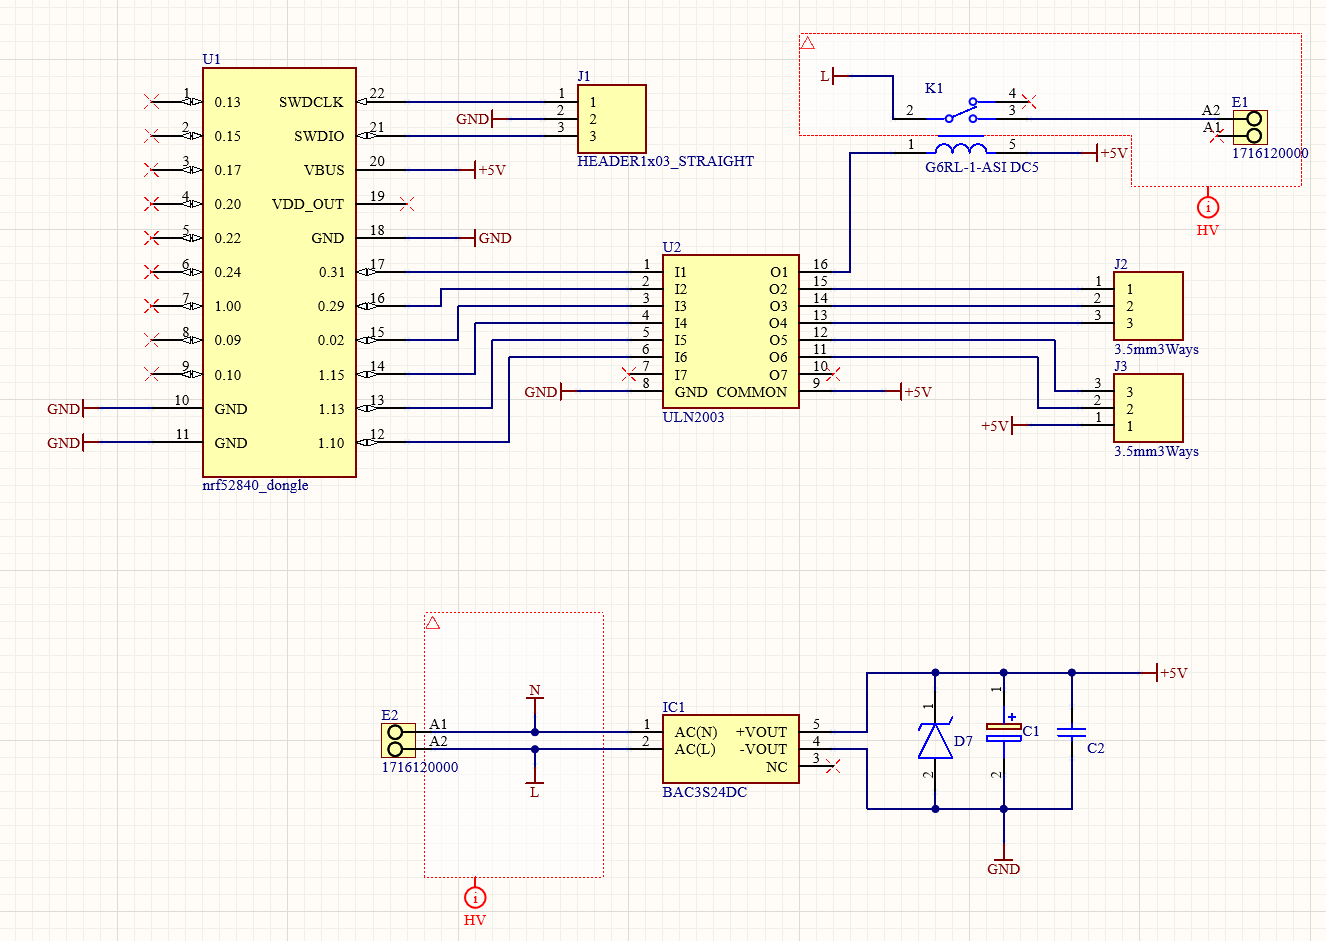
\includegraphics[width=\textwidth]{img/bapschematics.png}
    \caption{Blind Access Point schematic diagram}
    \label{fig:bapschematics}
\end{figure}
\noindent
I equip this device with one of the smallest AC/DC converter power supply (muRata BAC3S05DC) available on the market, which converts 230\,\si{\volt} mains voltage to 5\,\si{\volt} DC. With a 1x1 inch size and a maximum power rating of 3\,\si{\watt}, it is ideal for powering small devices. This module is shown in the lower half of Figure \ref{fig:bapschematics}. To the 5\,\si{\volt} output of the module I design a 7\,\si{\volt} suppressor diode (transient voltage protection), a 220\,\si{\micro\farad} tantalum capacitor (smoothing capacitor) and a 100\,\si{\nano\farad} filter capacitor, but these are also included in the power supply so they are optional.
I solve the switching of the lamp with a 5\,\si{\volt} relay, which connects the phase wire of the module to the lamp. This is important because, if wired correctly, the user's life is not at risk if he accidentally touches the phase point when changing a bulb with the lamp off. The wiring diagram shows the two blocks marked with HV, which is significant as there should be a minimum distance of 1.3\,\si{\milli\metre} between the phase and zero conductor, thus forming an Altium rule.


\subsection{Test panel assembly and software development}
\begin{figure}[!htb]
    \centering
    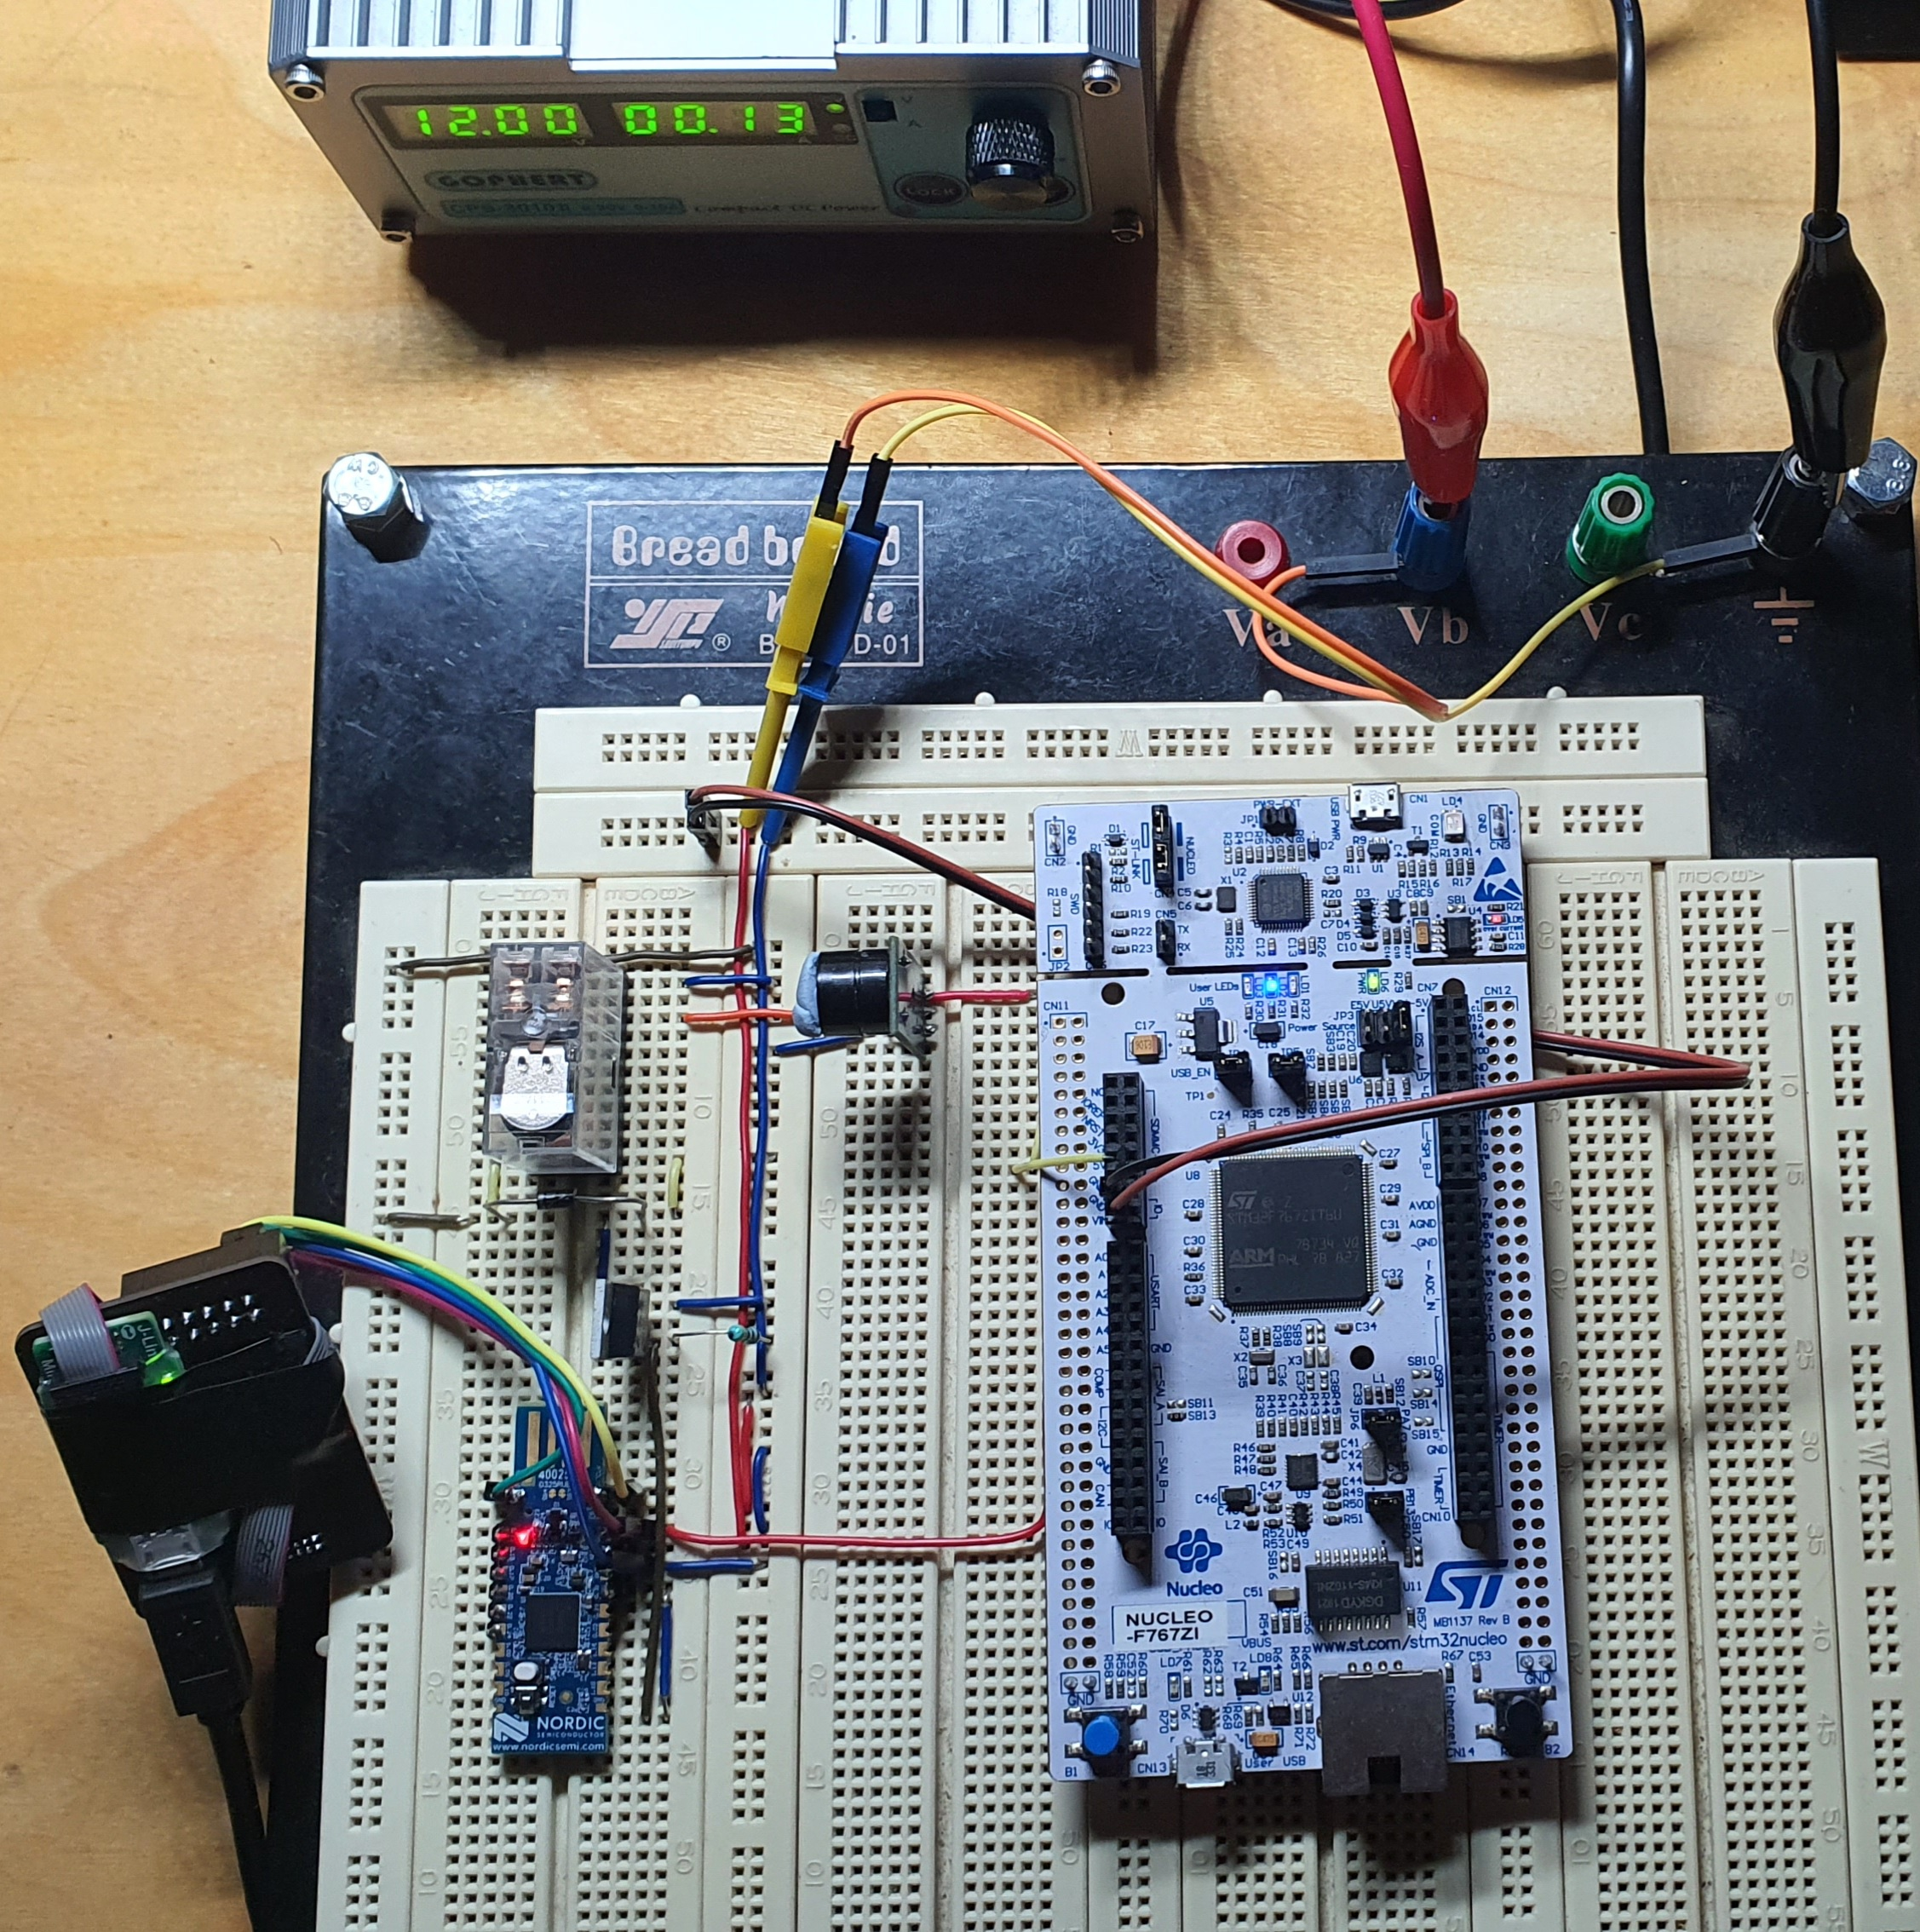
\includegraphics[width=\textwidth]{img/breadboard.jpg}
    \caption{Blind Access Point test panel assembly}
    \label{fig:breadboard}
\end{figure}
\noindent
Before designing the PCB, I created a breadboard concept, which is shown in Figure \ref{fig:breadboard}. I did not have the necessary components for the concept, so I substituted them with my tools at home and made the software accordingly. I wrote the software in the already familiar Zephyr, where two threads perform the device tasks. One thread handles the OpenThread and the Border Router address query, connection initiation and management functions and the special cases, what the programmer needs to handle. One such case is the \textit{callback} function that is called automatically after the device is connected, which gives information about the role of the device in the network. The other thread is responsible for checking the status of the lamp and switching the lamp. I implement this by having the device query the Border Router every half a second, then read the state of the lamp from the comment column of the device table from the database stored on the device, based on the device's eui64 ID if it is connected. In response, it sends a text to the device, which can be either "true" or "false". This is processed by the device and thus influences the state of the lamp.


\subsection{Blind Access Point PCB design}
In the PCB plan (shown in Figure \ref{fig:bap3D}) I tried to place the line voltage as far from the 5\,\si{\volt} line as possible. I designed a cut-out between the phase and zero conductor strips at the 230\,\si{\volt} part, so that I could create a sufficiently large spacing, since in dry air the breakdown voltage is approximately 1.3\,\si{\kilo\volt} per 1\,\si{\milli\metre}. In humid air, it can drop to 600\,\si{\volt}\cite{airbreakdownvoltage}, but this is still almost twice the maximum amplitude of the 230\,\si{\volt} mains voltage. I removed the solder mask from the high voltage section to ensure that solder mask would not absorb moisture, thus reduce the breakdown voltage.
In case one lamp is not enough, five outputs of 5\,\si{\volt} are available for a relay module. The control of the relays is solved by an IC (ULN2003) with six independent Darlington switches, which has flyback diodes on each output, thus ensuring a longer lifetime.

\begin{figure}[!htb]
    \centering
    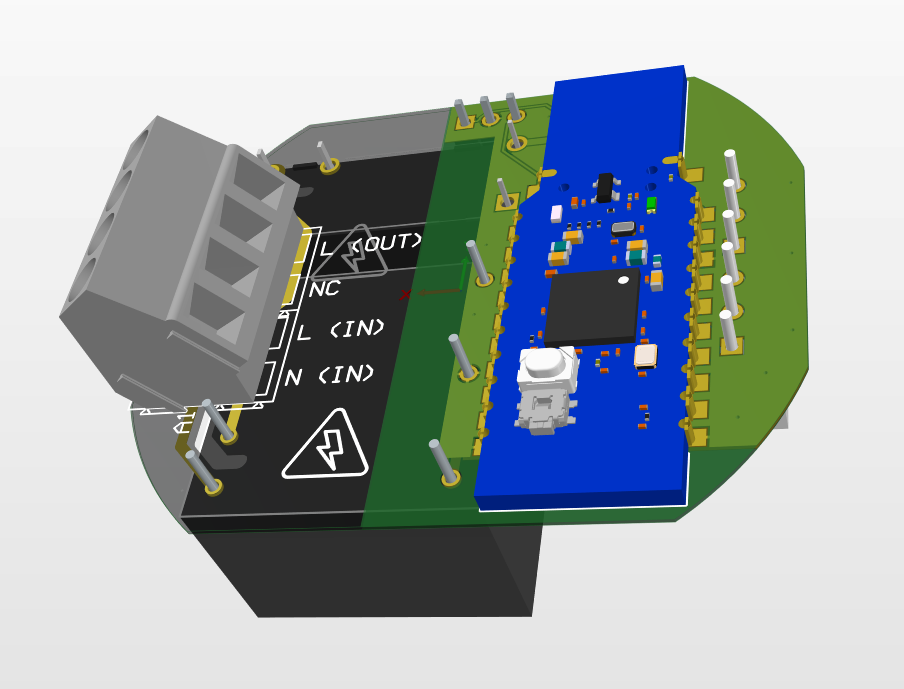
\includegraphics[width=\textwidth]{img/bap3d.png}
    \caption{Blind Access Point in 3D viewer}
    \label{fig:bap3D}
\end{figure}

